\chapter{Current Work}
\section{Frequency Sweep}
\paragraph{}
A frequency sweep, also referred to as frequency scanning or frequency modulation, is a deliberate variation of frequency over time. It entails the systematic alteration of a signal's frequency within a specified range, either continuously or in discrete steps. In our research experiment, we incorporate vibrometry measurements alongside OCT. This necessitates the use of a frequency sweep signal as input to a speaker. Currently, our setup lacks a dedicated Digital-to-Analog Converter (DAC) port to directly provide the sound signal. To circumvent this limitation, we are utilizing an external device to trigger a separate signal generator, which operates independently of the ThorImage software. Our objective is to develop code that seamlessly integrates with the C++ SDK and facilitates vibrometry experiments without the need for external interventions, streamlining the data acquisition process and enhancing the overall efficiency of our experiment.

\subsection*{MATLAB code for tone burst signal shown in Figure 4.1}
\begin{verbatim}
clear all;
close all;
clc;
% Parameters
frequency = 1; % Frequency of the wave (in Hz)
maxAmplitude = 5; % Maximum amplitude of the wave
duration = 10; % Duration of the wave (in seconds)
samplingRate = 44100; % Sampling rate (in Hz)
maxDuration = 7; % Duration of pause at max amplitude (in seconds)
% Time vector
t = linspace(0, duration, duration * samplingRate);
% Generate the wave
maxSamples = round(maxDuration * samplingRate); % No.of samples in maxduration
amplitude = [linspace(0, maxAmplitude, numel(t)/2-maxSamples/2), 
    maxAmplitude*ones(1, maxSamples), linspace(maxAmplitude,0, 
    numel(t)/2-maxSamples/2)];
wave = amplitude .* sin(2*pi*frequency*t);
% Plot the wave
plot(t, wave)
xlabel('Time (s)')
ylabel('Amplitude')
title('Tone burst signal at single frequency')
\end{verbatim}

\begin{figure}[H]\label{fig4.1}
\centering 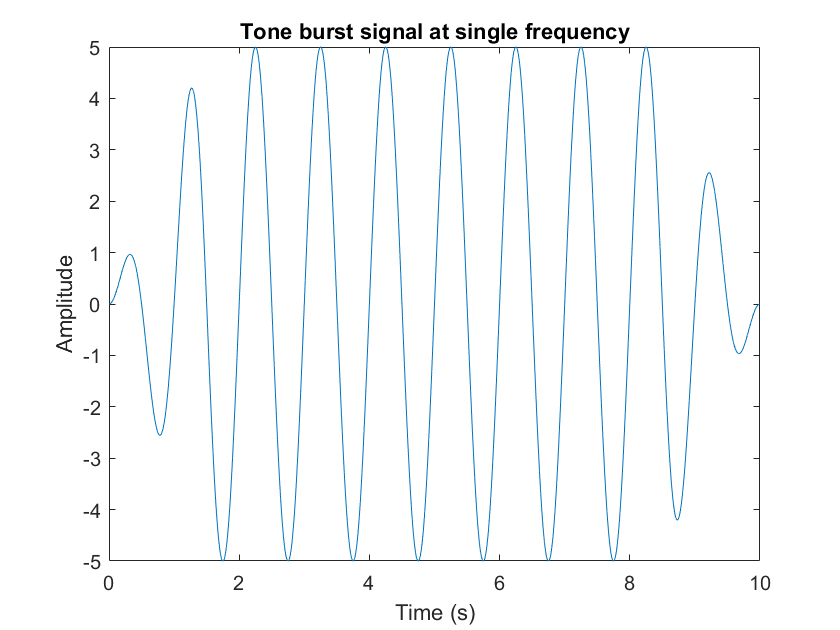
\includegraphics[scale=0.4]{Images/freqsweep1.png}
\caption{Tone burst signal for single frequency in time domain}
\end{figure}

\subsection*{MATLAB code for frequency sweep signal shown in Figure 4.2}
\begin{verbatim}
clear all;
close all;
clc;
% Parameters
frequencyA = 1; % Starting frequency
frequencyB = 5; % Ending frequency
numFrequencies = 10; % Number of frequencies
maxAmplitude = 5; % Maximum amplitude of the wave
Totduration = 10; % Total duration of the wave (in sec)
dutycycle = 0.8; % duty cycle for single frequency
samplingRate = 44100; % Sampling rate (in Hz)
maxDuration = 7; % Duration of pause at max amplitude (in sec)
%duty cycle allotment
duration = dutycycle*Totduration; % duration of wave (in sec)
Noduration = (1-dutycycle)*Totduration; % duration of free time
% Time vector
t = linspace(0, Totduration, Totduration * samplingRate);
% Calculate frequency step
frequencyStep = (frequencyB - frequencyA) / (numFrequencies - 1);
% Initialize the waveform
wave = zeros(1, numel(t) * numFrequencies);
% Generate waves for each frequency
for i = 1:numFrequencies
    % Calculate current frequency
    currentFrequency = frequencyA + (i-1) * frequencyStep;
    % Generate the wave
    maxSamples = round(maxDuration * samplingRate); 
        % No.of samples in maxduration
    nodursamples = round(Noduration * samplingRate); 
        % Number of samples for the 0% duty cycle
    amplitude = [linspace(0, maxAmplitude, numel(t)/2-maxSamples/2-
        nodursamples/2), maxAmplitude*ones(1, maxSamples), 
        linspace(maxAmplitude,0,numel(t)/2-maxSamples/2-
        nodursamples/2), maxAmplitude*zeros(1, nodursamples)];
    currentWave = amplitude .* sin(2*pi*currentFrequency*t);
    % Accumulate the waveforms
    wave((i-1)*numel(t)+1:i*numel(t)) = currentWave;
end
t1 = linspace(0,numFrequencies*Totduration,
    numFrequencies*Totduration*samplingRate);
% Plot the combined wave
plot(t1, wave)
xlabel('Time (s)')
ylabel('Amplitude')
title('frequency sweep signal')
\end{verbatim}

\begin{figure}[H]\label{fig4.2}
\centering 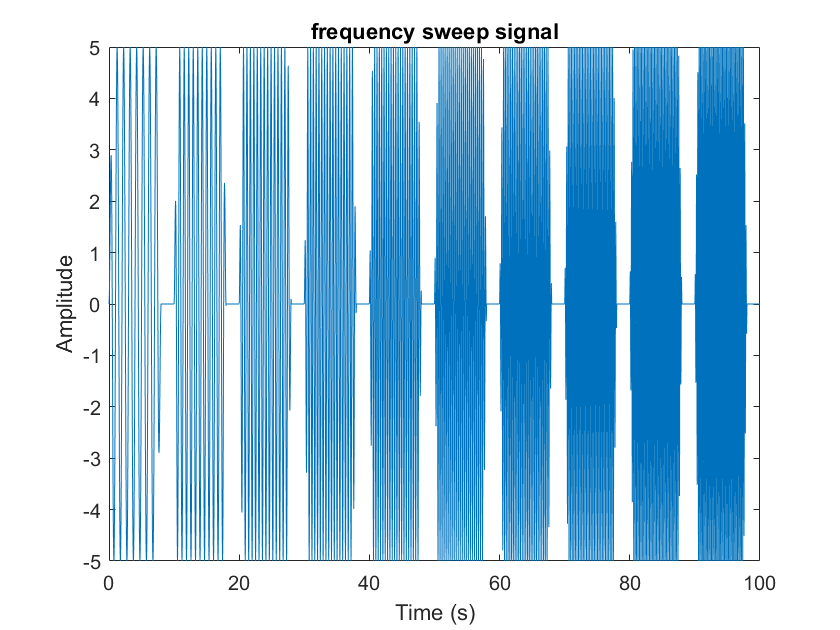
\includegraphics[scale=0.4]{Images/freqsweep2.png}
\caption{frequency sweep signal}
\end{figure}

\section{C++ SDK}
\paragraph{}
There are four distinct code files within the C++ SDK, each designed to serve specific functionalities. Let's delve into a detailed discussion of each of these files.

\subsection{Simple Spectral Radar}
\paragraph{}
This file comprises fundamental demonstration programs that illustrate how to utilize the SDK.

\subsubsection{Simple Measurement}
\paragraph{}
This code generates a simple B-scan pattern, allowing users to define the desired range and number of A-scans. Subsequently, it saves the processed data to a CSV file at the specified location.

\subsubsection{Export Data and Image}
\paragraph{}
This code generates a basic B-scan pattern, permitting users to define the desired range and number of A-scans. Additionally, it saves the processed data to both a CSV file and an image file at the specified location.

\subsubsection{Averaging and Imaging Speed}
\paragraph{}
To enhance image quality, this code offers two options. The first option is to reduce the scan speed, which increases the integration cycle time, resulting in improved image quality. The second option involves performing A and B-scans multiple times and calculating averages. This code executes these operations and generate a B-scan pattern and then saves the processed image at a user-specified location.

\subsubsection{Volume Scan Pattern}
\paragraph{}
This code creates a volumetric scan pattern, enabling users to specify the number of A-scans, B-scans, and the desired level of B-scan averaging.

\subsubsection{Modify Scan Pattern}
\paragraph{}
In a basic measurement setup, this code initially establishes horizontal scan patterns typically centered at (0.0, 0.0). It offers functions for rotation and zoom around the origin, followed by a shift of the origin point. Subsequently, a B-scan pattern is generated with these adjustments.

\subsubsection{Continuous Measurement}
\paragraph{}
This code offers functionality to contunously acquire multiple B-scans for the same defined B-scan pattern

\subsection{Create Free Form Scan Patterns}
\paragraph{}
This code serves as a demonstration of how to generate scan points using the Freeform Scan Pattern feature, which can be applied within ThorImage or integrated into other functions within the SDK. These scan points are formatted and saved in a standard TXT file, allowing for easy modification. The code enables the creation of scan pattern points for simple geometric shapes like circles, triangles, crosses, and more.

\subsection{External Processing}
\paragraph{}
This code offers a simple example of an external processing routine that reads raw OCT data from an input file, applies a basic processing step to each B-scan, and then writes the processed data to an output file. Its primary purpose is to showcase how external processing can be integrated with ThorImage to facilitate custom data manipulation.

\subsection{Advanced Spectral Radar}
\subsubsection{Write OCT File}
\paragraph{}
This program lets us to write data acquired with the SDK to an oct-file which can be viewed with ThorImageOCT. The generated oct-file is then stored in the same folder where the SDK is present.

\subsubsection{Read OCT File}
\paragraph{}
This program lets us read an oct-file with the SDK which has been acquired and saved with ThorImageOCT.

\subsubsection{Write OCT File with free form scan pattern}
\paragraph{}
In contrast to the previous Write OCT file function, this code allows for the utilization of custom, free-form scan patterns such as circles, triangles, or crosses, rather than being restricted to the standard straight-line pattern. Subsequently, the program generates an OCT file that can be easily read via ThorImage for further analysis and visualization.

\newpage
\subsubsection{Processing Chain}
\paragraph{}
The processing chain comprises multiple sequential steps, and using the SDK, it's feasible to access and work with the processed data at various intermediate stages, not just at the final step. This function empowers us to process the raw data acquired from the scan pattern using our customized processing routines. These routines encompass examples such as "Offset corrected spectrum," "Spectrum output," "DC corrected spectrum output," "Apodized spectrum output," and more.

\subsubsection{Advanced Modification of Scan Pattern}
\paragraph{}
Using this code, it's possible to construct a scan pattern that consists of multiple consecutive B-scans acquired directly one after another. All B-scans within this pattern must have the same number of A-scans, enabling the creation of patterns involving rotating B-scans. One method to achieve such a pattern is to initially create a volume pattern and subsequently modify it using the functions `shiftScanPatternEx` and `rotateScanPatternEx`. These functions allow for the shifting and rotation of individual B-scans within the volume pattern. This code demonstrates the usage of the `rotateScanPatternEx` function, while the use of `shiftScanPatternEx` follows a similar approach.

\subsubsection{Free Form Scan Pattern}
\paragraph{}
The freeform scan pattern functions provide users with the flexibility to generate 2D and 3D scan patterns of virtually any shape. These patterns can be defined using two distinct approaches. Firstly, users can specify only the edge points of the pattern, relying on interpolation methods to calculate the actual scan points within. Alternatively, users have the option to manually create all scan positions, which will be utilized exactly as provided without any interpolation. 

\subsubsection{Removing Apo from Scan Pattern}
\paragraph{}
In certain scenarios, it can be beneficial to eliminate the acquisition of additional apodization spectra during the processing routine to expedite the acquisition process. This can be achieved by conducting the acquisition of these apodization spectra before initiating the measurement, subsequently using them in the processing chain. By setting the number of apodization spectra to zero, no apodization is applied during the scan, resulting in faster scanning. Additionally, this reduces the time required for the scanner to reach the starting position of each scan, as only one flyback time is needed instead of two in the absence of apodization spectra acquisition.

\subsubsection{Doppler OCT}
\paragraph{}
This code initially executes a standard processing routine to generate a B-scan pattern. Subsequently, it performs additional processing steps to perform Doppler OCT imaging. Users have the flexibility to define the output parameters for the Doppler processing and specify averaging parameters for the processing routine. Ultimately, the code carries out Doppler processing to obtain Doppler OCT images.

\subsubsection{Speckle Variance OCT}
\paragraph{}
This code begins by running a standard processing routine to create a volume scan pattern. It then proceeds to execute additional processing steps aimed at conducting Speckle Variance OCT imaging. Users are given the option to define averaging parameters for the processing routine as needed. Finally, the code calculates the speckle variance and exports the resulting data in CSV format to a user-specified location.

\subsubsection{External Trigger Modus}
\paragraph{}
This code offers the functionality to externally trigger the acquisition of A-scans. This capability allows users to synchronize measurements from various modalities, such as vibrometry and synchronized positioning, with an OCT measurement. It's crucial to ensure that the trigger signal initiates after the `startMeasurement()` function and concludes after the `stopMeasurement()` function. This demo program provides clear guidance on when to apply and disable the external trigger for proper synchronization.

% \subsubsection{Batch Measurement with polarization adjustment}
% \paragraph{}
% This demonstration captures a batch of B-scans, with each B-scan using a different setting of the polarization control. The resulting images are then exported to the directory \begin{verbatim}"C:\OCTExport\" \end{verbatim} with filenames like "demo_batch_*.png," where the asterisk (*) represents the specific image index. Each polarization retarder setting will go through "n" POLARIZATION_STEPS, resulting in a total of n*n images being captured and exported.

% \subsubsection{Automatic reference and amplification adjustment}
% \paragraph{}

% \subsubsection{Image field calibration}
% \paragraph{}

% \subsubsection{Ring light adjustment}
% \paragraph{}


\subsection{Validation experiment}
\paragraph{}
We acquired a simple B-scan pattern using ThorImage software and recreated the identical setup using the C++ SDK. Subsequently, we processed the data obtained through the SDK to generate images for a comparative analysis with those generated by ThorImage. The findings from this comparison are displayed below.

\paragraph{}
As depicted in Figure 4.4, we observe a B-scan with range of 2.19 mm and a depth of 3.56 mm. Within this range, 10,000 pixels correspond to 10,000 A-scans. To replicate a similar scan pattern as seen in ThorImage software, we provided the C++ SDK's "Modify Scan Pattern" function with these parameters, accounting for a noticeable origin shift present in ThorImage. The resulting scan pattern from the SDK was saved in a CSV file, a snapshot of which is displayed in Figure 4.5. By comparing Figure 4.4 and Figure 4.5, we observe that the depth information, in regions with multiple layers, appears to align between the ThorImage-generated data and that obtained through the SDK.

% \pagebreak

\begin{figure}[H]\label{fig4.3}
\centering 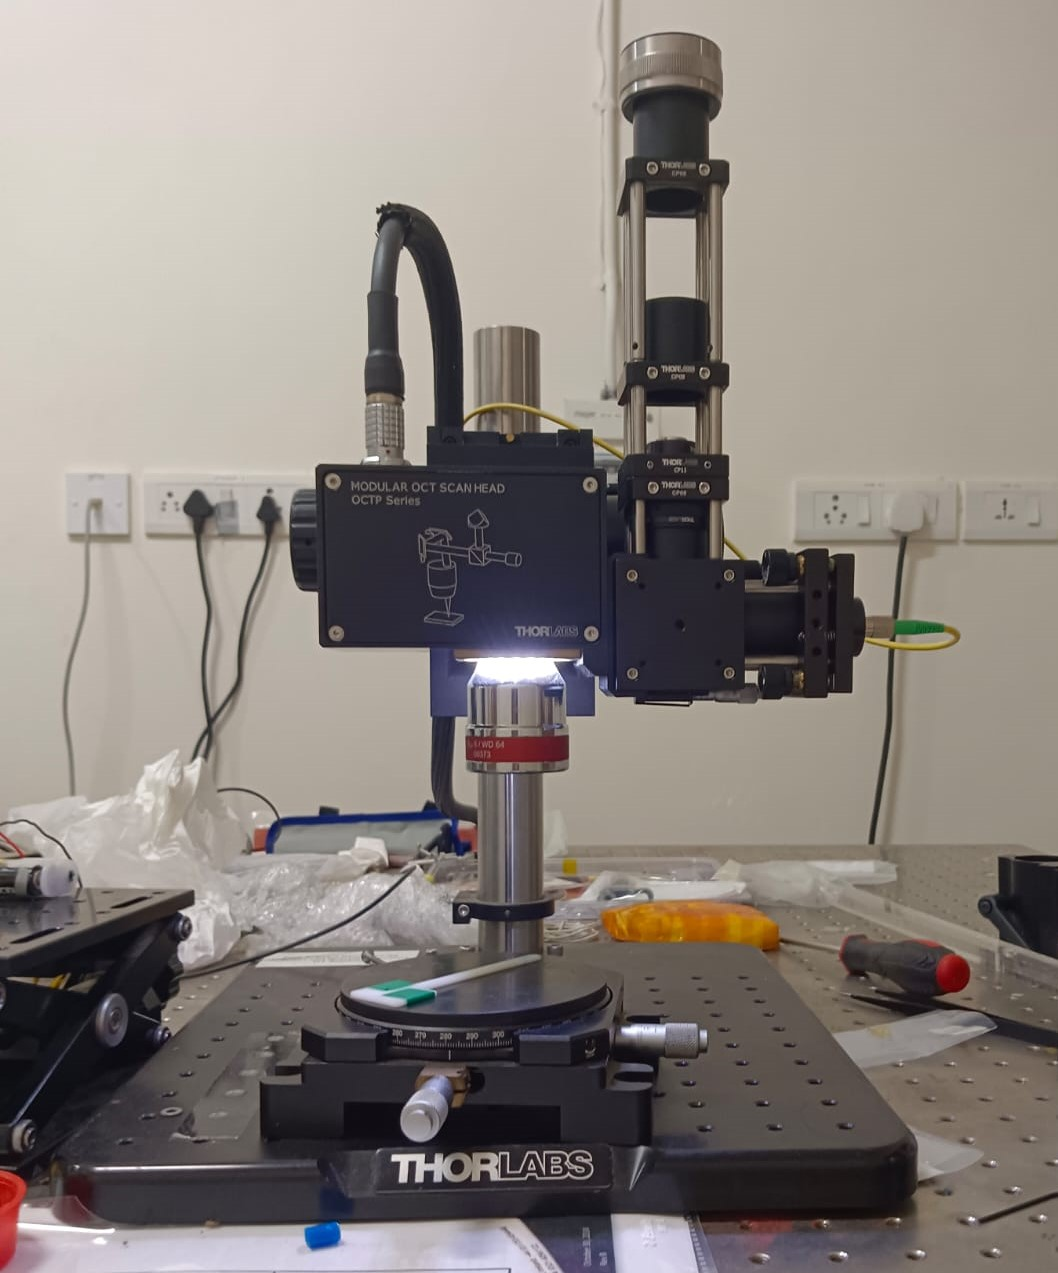
\includegraphics[scale=0.2]{Images/ExptSetup.jpg}
\caption{Validation Experimental Setup}
\end{figure}

\begin{figure}[H]\label{fig4.4}
\centering 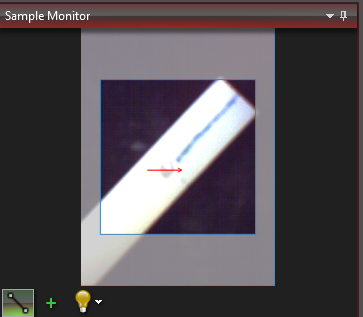
\includegraphics[scale=0.5]{Images/ScanPattern_ThorImage2.PNG}
\caption{View of the sample for the experiment}
\end{figure}

\begin{figure}[H]\label{fig4.5}
\centering 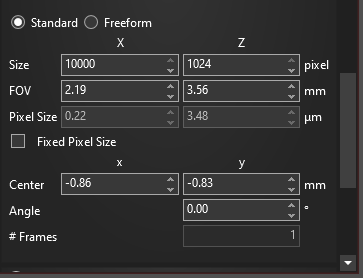
\includegraphics[scale=0.5]{Images/ScanPattern_ThorImage1.PNG}
\caption{Scan pattern specified in ThorImage software}
\end{figure}

\begin{figure}[H]\label{fig4.6}
\centering 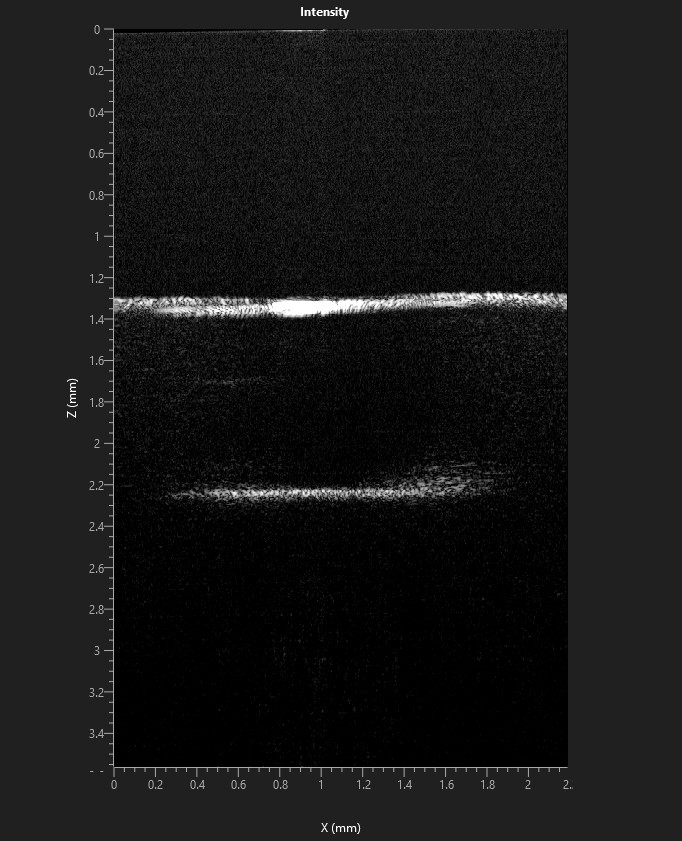
\includegraphics[scale=0.25]{Images/OCT_Image_ThorImage.PNG}
\caption{Obtained OCT image using ThorImage software}
\end{figure}

\begin{figure}[H]\label{fig4.7}
\centering 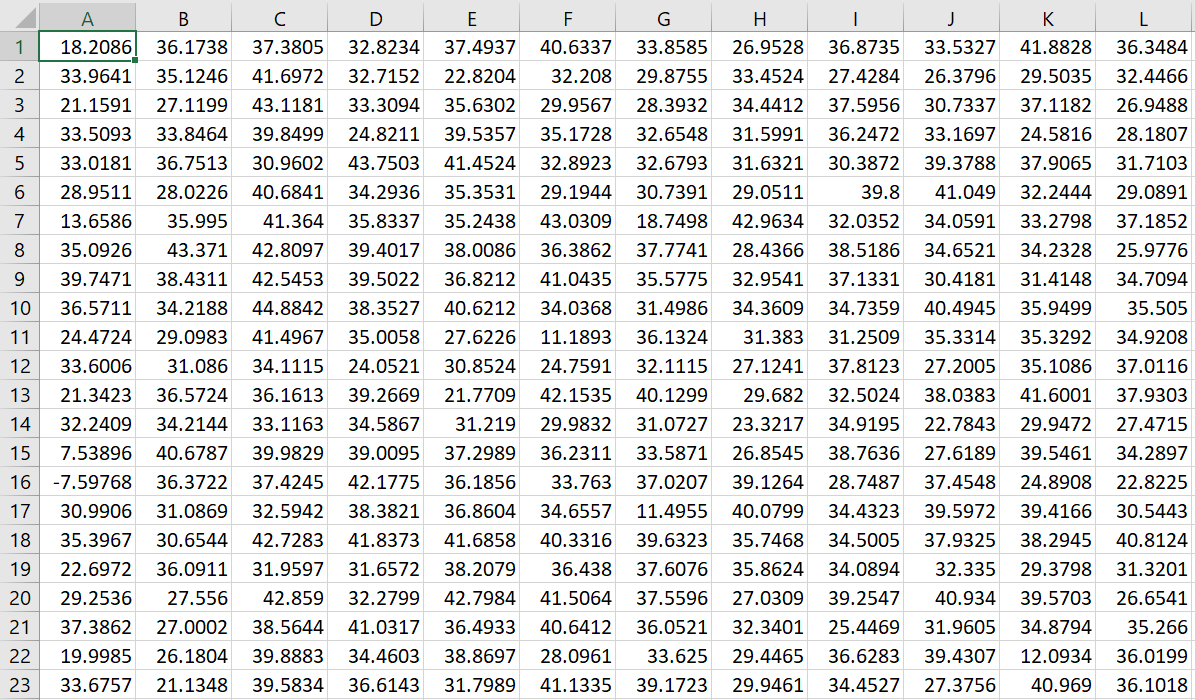
\includegraphics[scale=0.35]{Images/test_oct_xls.PNG}
\caption{Intensity data obained using SDK}
\end{figure}

\begin{figure}[H]\label{fig4.8}
\centering 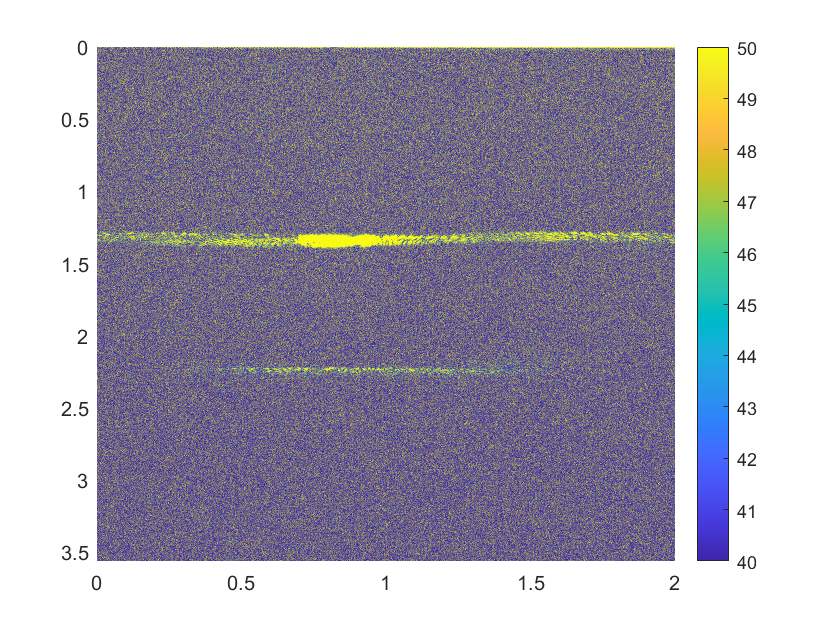
\includegraphics[scale=0.35]{Images/OCT_Image_SDK.PNG}
\caption{Post processed OCT image from data obtained using SDK}
\end{figure}

\begin{figure}[H]\label{fig4.9}
\centering 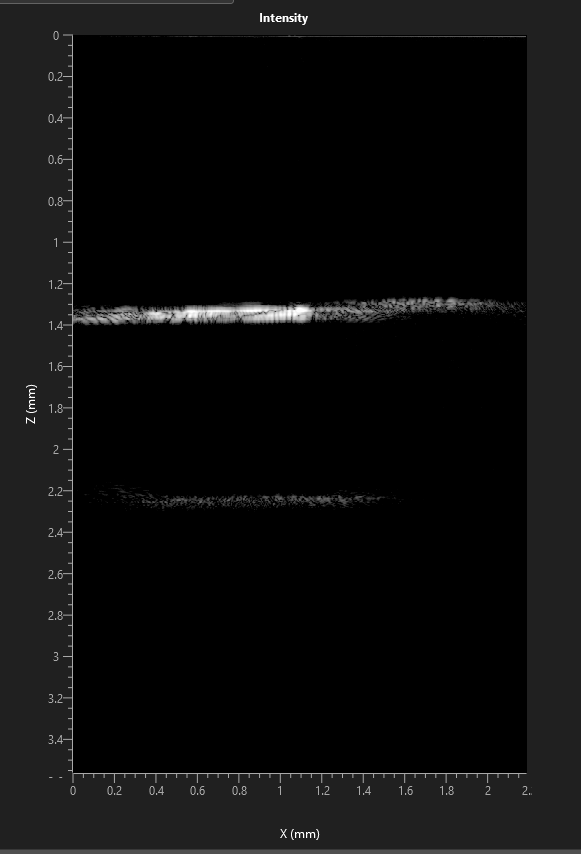
\includegraphics[scale=0.35]{Images/OCT_image_from_SDK.PNG}
\caption{.oct file obtained using SDK opened in ThorImage}
\end{figure}

% \newpage 
\section{Handheld Otoscope}